\clearpage

\section{Network components}\label{network_components}

\subsection{Link architecture}

Links are basically physical point-to-point connections ensured by the transmission systems between two adjacent nodes.
These links can be composed of one or more transmission systems, where it starts and ends at the node and has the function of transporting a WDM signal between the directly connected nodes \cite{book07}\cite{ramas2010}. Signals are transmitted through a pair of fibers that require bidirectional communication.
Transmission systems contain optical amplifiers at an expected distance (span) in order to increase signal strength thus allowing reliable signal detection \cite{tesevasco}.

\subsection{Node architecture}

In the node are performed enough operations thus requiring a lot of hardware, consequently, are considered the element of a more expensive optical transport network.
In optical networks these nodes are composed of three structures: modules, shelves and rack. The modules contain optical and electrical components to perform functions such as encapsulation and wavelength assignment and these can contain multiple ports. The shelves are designed to support different modules so that they can be assembled. Finally, the rack has the function of supplying power to the shelves \cite{tesevasco,teserui}.

\begin{figure}[h!]
\centering
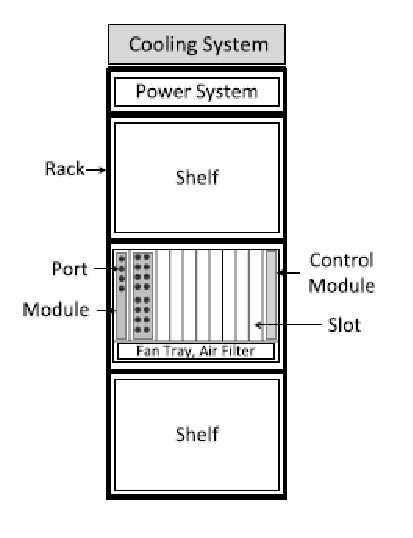
\includegraphics[width=5cm]{sdf/reference_network/figures/node}
\caption{Schematic of a node where we can see the main components \cite{teserui,tesevasco}.}
\label{node_struct}
\end{figure}

\section{Network topologies}\label{network_topologies}

\subsection{Physical topology}

A physical topology is defined by a set of nodes and edges that characterize the network. The nodes are where we can find the elements of the network. Already the edges are the physical interconnection between these nodes where in this case correspond to optical fibers.
Some of the common physical topologies are mesh, ring, and star topology \cite{aulas2}\cite{teselisboa}.

\subsection{Logical topology}

Fundamentally, the logical topology represents how the flow of traffic on the network occurs. This flow can be described in terms of traffic requests, or logical links.
Logical topologies can be represented by traffic arrays where the elements of the array entry represent the number of client traffic units that flow between the source node and the destination node.
If you know all traffic requests we can say that we are dealing with static traffic. In the situation where all requests for traffic are not known, this traffic is said to be dynamic \cite{aulas2}\cite{teselisboa}.

\section{Transport modes}\label{transport_mode}

\subsection{Opaque transport mode}\label{opaque}

A network configured in opaque transport mode performs OEO conversions on each intermediate node because of the need for converting to electronic domain \cite{book07}.
An advantage in this way is that it eliminates the accumulation of physical deficiencies and allows full flexibility in the exchange and removal of customer signals \cite{teserui}.
The optical and physical topologies are the same, causing each traffic route to match the link-to-link path imposed by fiber optics between each intermediate node to the destination \cite{tesevasco,opaque}.\\

\subsection{Transparent transport mode}\label{transparent}

In transparent transport mode, a route is only defined between source and destination nodes always in the optical domain \cite{book07}. In this mode the physical and optical topologies are different \cite{tesevasco}.
Since this type of network performs the OEO conversion only at the end nodes of the path, the capacity's utilization of the wavelength channels is restricted to the client signals with the same endpoints \cite{teserui,transparent}.\\

\subsection{Translucent transport mode}\label{translucent}
The translucent mode of transport is a combination of the other two transport modes taking the respective advantages of both \cite{book07}. Therefore in this mode of transport the physical and optical topologies are different, the latter having several solutions \cite{tesevasco}. Regarding the OEO conversion in this case it is done in some intermediate places before arriving at its destination \cite{teserui}.
As far as grooming is concerned, translucent mode uses a multi-hop scheme where client signals with different source and destination nodes can share the same lightpath \cite{zhu}.

\section{Reference network}\label{reference_network}

\subsection{Physical topology}\label{Reference_Network_Topology}

The networks are distinguished by different physical topologies.
A physical topology is defined by a set of nodes and links, which physically interconnect the nodes, that characterize the network.
In this specific case the physical topology can be seen in figure \ref{physical_top_ref_net} where it is possible to see that the reference network consists of 6 nodes and 8 bidirectional links.
Besides this layout of links and nodes will also need to know the average length of the links.
This value varies depending on the length of each link so it will be necessary to define all distances between the respective nodes.
Finally, it is also necessary to indicate the total traffic used in this network so the ODU matrices will be created.\\

\begin{figure}[h!]
\centering
\includegraphics[width=\textwidth]{sdf/reference_network/figures/RedeTeste}
\caption{Physical topology of the reference network.}
\label{physical_top_ref_net}
\end{figure}

\vspace{11pt}
The distance matrix for this reference network is the same regardless of its associated traffic.
The values indicated in the distance matrix, referred below, are expressed in kilometers (Km) and, as it could not be otherwise, this matrix is symmetric because the distance from $node1$ to $node2$ must be the same as $node2$ to $node1$.\\

\[
Dist=
  \begin{bmatrix}
    0 & 460 & 663 & 0 & 0 & 0 \\
    460 & 0 & 75 & 684 & 0 & 0 \\
    663 & 75 & 0 & 0 & 890 & 0 \\
    0 & 684 & 0 & 0 & 103 & 764 \\
    0 & 0 & 890 & 103 & 0 & 361 \\
    0 & 0 & 0 & 764 & 361 & 0
  \end{bmatrix}
\]

\newpage
For this case study we have to take into consideration the table \ref{table_ref_net} because in it we can see the values of the variables associated with this network.

\begin{table}[h!]
\centering
\begin{tabular}{|| c | c | c||}
 \hline
 Constant & Description & Value \\
 \hline\hline
 N & Number of nodes & 6 \\
 L & Number of bidirectional links & 8 \\
 <$\delta$> & Node degree & 2.667 \\
 <len> & Mean link length (km) & 500 \\
 <h> & Mean number of hops for working paths & 1.533 \\
 <h'> & Mean number of hops for backup paths & 2.467 \\
 \hline
\end{tabular}
\caption{Table of reference network values.}
\label{table_ref_net}
\end{table}


\subsection{Traffic network}\label{Reference_Network_Traffic}

For a better interpretation of the later results we will assume three traffic scenarios for this network being the first scenario with a low traffic, the second with a medium traffic and a last one with a high traffic.
For each scenario it will be necessary to create different traffic matrices and to know the traffic of the network we will use five matrices of traffic.
These traffic matrices are represented by ODU0, ODU1, ODU2, ODU3 and ODU4 where each one has a certain bit rate.
The ODU0 corresponds to 1.25 Gbits/s, the ODU1 corresponds to 2.5 Gbits/s, the ODU2 corresponds to 10 Gbits/s, the ODU3 corresponds to 40 Gbits/s and finally the ODU4 corresponds to 100 Gbits/s \cite{alcatel}.
As we can see below, these matrices are bi-directional because they are symmetric arrays and as such, the traffic sent in a certain direction must be the same traffic sent in that opposite direction.

\subsubsection{Low traffic scenario}\label{low_scenario}

For this scenario, as it is intended low traffic, is decided that will have an average of less than 100 Gbits/s per node, preferring a total of traffic of the network of 0.5 Tbits/s.
After defining the traffic it is necessary to divide this traffic by the different ODU's thus creating several traffic matrices.
The traffic matrices for this scenario are:

\[
ODU0=
  \begin{bmatrix}
    0 & 5 & 1 & 3 & 1 & 3 \\
    5 & 0 & 0 & 1 & 5 & 0 \\
    1 & 0 & 0 & 1 & 4 & 1 \\
    3 & 1 & 1 & 0 & 1 & 1 \\
    1 & 5 & 4 & 1 & 0 & 3 \\
    3 & 0 & 1 & 1 & 3 & 0
  \end{bmatrix}
\qquad ODU1=
  \begin{bmatrix}
    0 & 2 & 4 & 2 & 0 & 5 \\
    2 & 0 & 0 & 3 & 1 & 1 \\
    4 & 0 & 0 & 1 & 1 & 0 \\
    2 & 3 & 1 & 0 & 1 & 3 \\
    0 & 1 & 1 & 1 & 0 & 1 \\
    5 & 1 & 0 & 3 & 1 & 0
  \end{bmatrix}
\]
\[
ODU2=
  \begin{bmatrix}
    0 & 1 & 1 & 1 & 0 & 0 \\
    1 & 0 & 0 & 0 & 1 & 0 \\
    1 & 0 & 0 & 1 & 1 & 0 \\
    1 & 0 & 1 & 0 & 1 & 0 \\
    0 & 1 & 1 & 1 & 0 & 1 \\
    0 & 0 & 0 & 0 & 1 & 0
  \end{bmatrix}
\qquad ODU3=
  \begin{bmatrix}
    0 & 0 & 0 & 0 & 0 & 0 \\
    0 & 0 & 1 & 0 & 0 & 1 \\
    0 & 1 & 0 & 0 & 1 & 0 \\
    0 & 0 & 0 & 0 & 0 & 0 \\
    0 & 0 & 1 & 0 & 0 & 0 \\
    0 & 1 & 0 & 0 & 0 & 0
  \end{bmatrix}
\]
\[
ODU4=
  \begin{bmatrix}
    0 & 0 & 0 & 0 & 0 & 0 \\
    0 & 0 & 0 & 0 & 0 & 1 \\
    0 & 0 & 0 & 0 & 0 & 0 \\
    0 & 0 & 0 & 0 & 0 & 0 \\
    0 & 0 & 0 & 0 & 0 & 1 \\
    0 & 1 & 0 & 0 & 1 & 0
  \end{bmatrix}
\]

Through these ODUs, we can calculate and confirm the total network traffic for the low traffic scenario: \\

$T_1^0$ = 60x1.25 = 75 Gbits/s \qquad
$T_1^1$ = 50x2.5 = 125 Gbits/s \qquad
$T_1^2$ = 16x10 = 160 Gbits/s \\

$T_1^3$ = 6x40 = 240 Gbits/s \quad
$T_1^4$ = 4x100 = 400 Gbits/s \\

$T_{1}$ = 75 + 125 + 160 + 240 + 400 = 1000 Gbits/s \qquad
$T$ = 1000/2 = \textbf{0.5 Tbits/s}\\

Where the variable $T_1^x$ represents the unidirectional traffic of the ODUx. The variable $T_{1}$ represents the total of unidirectional traffic that is injected into the network and finally the variable $T$ represents the total of bidirectional traffic.\\

Once the traffic matrices are defined we will focus on the logical network topology. In the following figures we can see the logical topologies of the different ODUs created based on the respective matrices.\\

\begin{figure}[h!]
\centering
\includegraphics[width=9cm]{sdf/ilp/opaque_survivability/figures/logical_topology_ODU0_low}
\caption{ODU0 logical topology defined by the ODU0 traffic matrix in low scenario.}
\label{logical_ODU0_low}
\end{figure}
\newpage
\begin{figure}[h!]
\centering
\includegraphics[width=9cm]{sdf/ilp/opaque_survivability/figures/logical_topology_ODU1_low}
\caption{ODU1 logical topology defined by the ODU1 traffic matrix in low scenario.}
\label{logical_ODU1_low}
\end{figure}

\begin{figure}[h!]
\centering
\includegraphics[width=9cm]{sdf/ilp/opaque_survivability/figures/logical_topology_ODU2_low}
\caption{ODU2 logical topology defined by the ODU2 traffic matrix in low scenario.}
\label{logical_ODU2_low}
\end{figure}

\begin{figure}[h!]
\centering
\includegraphics[width=9cm]{sdf/ilp/opaque_survivability/figures/logical_topology_ODU3_low}
\caption{ODU3 logical topology defined by the ODU3 traffic matrix in low scenario.}
\label{logical_ODU3_low}
\end{figure}

\begin{figure}[h!]
\centering
\includegraphics[width=9cm]{sdf/ilp/opaque_survivability/figures/logical_topology_ODU4_low}
\caption{ODU4 logical topology defined by the ODU4 traffic matrix in low scenario.}
\label{logical_ODU4_low}
\end{figure}

\subsubsection{Medium traffic scenario}\label{medium_traffic_scenario}

Now, in this scenario, a significant increase in traffic is already assumed. For this it is decided that it will have an average of less than 1 Tbits/s per node, prefiguring a total of 5 Tbits/s network traffic.
In the next step the division of the traffic defined previously by the different ODU's is made, therefore creating several matrices of traffic.
The traffic matrices for this scenario are:

\[
ODU0=
  \begin{bmatrix}
    0 & 50 & 10 & 30 & 10 & 30 \\
    50 & 0 & 0 & 10 & 50 & 0 \\
    10 & 0 & 0 & 10 & 40 & 10 \\
    30 & 10 & 10 & 0 & 10 & 10 \\
    10 & 50 & 40 & 10 & 0 & 30 \\
    30 & 0 & 10 & 10 & 30 & 0
  \end{bmatrix}
\quad ODU1=
  \begin{bmatrix}
    0 & 20 & 40 & 20 & 0 & 50 \\
    20 & 0 & 0 & 30 & 10 & 10 \\
    40 & 0 & 0 & 10 & 10 & 0 \\
    20 & 30 & 10 & 0 & 10 & 30 \\
    0 & 10 & 10 & 10 & 0 & 10 \\
    50 & 10 & 0 & 30 & 10 & 0
  \end{bmatrix}
\]
\[
ODU2=
  \begin{bmatrix}
    0 & 10 & 10 & 10 & 0 & 0 \\
    10 & 0 & 0 & 0 & 10 & 0 \\
    10 & 0 & 0 & 10 & 10 & 0 \\
    10 & 0 & 10 & 0 & 10 & 0 \\
    0 & 10 & 10 & 10 & 0 & 10 \\
    0 & 0 & 0 & 0 & 10 & 0
  \end{bmatrix}
\quad ODU3=
  \begin{bmatrix}
    0 & 0 & 0 & 0 & 0 & 0 \\
    0 & 0 & 10 & 0 & 0 & 10 \\
    0 & 10 & 0 & 0 & 10 & 0 \\
    0 & 0 & 0 & 0 & 0 & 0 \\
    0 & 0 & 10 & 0 & 0 & 0 \\
    0 & 10 & 0 & 0 & 0 & 0
  \end{bmatrix}
\]
\[
ODU4=
  \begin{bmatrix}
    0 & 0 & 0 & 0 & 0 & 0 \\
    0 & 0 & 0 & 0 & 0 & 10 \\
    0 & 0 & 0 & 0 & 0 & 0 \\
    0 & 0 & 0 & 0 & 0 & 0 \\
    0 & 0 & 0 & 0 & 0 & 10 \\
    0 & 10 & 0 & 0 & 10 & 0
  \end{bmatrix}
\]

Once again, through these ODU's we can calculate and confirm the total network traffic for the medium traffic scenario:\\

$T_1^0$ = 600x1.25 = 750 Gbits/s \quad
$T_1^1$ = 500x2.5 = 1205 Gbits/s \quad
$T_1^2$ = 160x10 = 1600 Gbits/s \\

$T_1^3$ = 60x40 = 2400 Gbits/s \quad
$T_1^4$ = 40x100 = 4000 Gbits/s \\

$T_{1}$ = 750 + 1250 + 1600 + 2400 + 4000 = 10000 Gbits/s \qquad
$T$ = 10000/2 = \textbf{5 Tbits/s}\\

Again, focusing on the logical topology of the network, we can see the different topologies created based on the respective matrices.
\newpage
\begin{figure}[h!]
\centering
\includegraphics[width=9cm]{sdf/ilp/opaque_survivability/figures/logical_topology_ODU0_medium}
\caption{ODU0 logical topology defined by the ODU0 traffic matrix in medium scenario.}
\label{logical_ODU0_medium}
\end{figure}

\begin{figure}[h!]
\centering
\includegraphics[width=9cm]{sdf/ilp/opaque_survivability/figures/logical_topology_ODU1_medium}
\caption{ODU1 logical topology defined by the ODU1 traffic matrix in medium scenario.}
\label{logical_ODU1_medium}
\end{figure}

\begin{figure}[h!]
\centering
\includegraphics[width=9cm]{sdf/ilp/opaque_survivability/figures/logical_topology_ODU2_medium}
\caption{ODU2 logical topology defined by the ODU2 traffic matrix in medium scenario.}
\label{logical_ODU2_medium}
\end{figure}

\begin{figure}[h!]
\centering
\includegraphics[width=9cm]{sdf/ilp/opaque_survivability/figures/logical_topology_ODU3_medium}
\caption{ODU3 logical topology defined by the ODU3 traffic matrix in medium scenario.}
\label{logical_ODU3_medium}
\end{figure}
\newpage
\begin{figure}[h!]
\centering
\includegraphics[width=9cm]{sdf/ilp/opaque_survivability/figures/logical_topology_ODU4_medium}
\caption{ODU4 logical topology defined by the ODU4 traffic matrix in medium scenario.}
\label{logical_ODU4_medium}
\end{figure}

\subsubsection{High traffic scenario}\label{high_traffic_scenario}

In the latter scenario it is considered to create a new increase of traffic leaving, in this way the network with a lot of traffic to carry. It is assumed a total of 10 Tbits/s network traffic.
In the next step using the different ODU's the division of the traffic is made, creating several matrices of traffic.
The traffic matrices for this scenario are:

\[
ODU0=
  \begin{bmatrix}
    0 & 100 & 20 & 60 & 20 & 60 \\
    100 & 0 & 0 & 20 & 100 & 0 \\
    20 & 0 & 0 & 20 & 80 & 20 \\
    60 & 20 & 20 & 0 & 20 & 20 \\
    20 & 100 & 80 & 20 & 0 & 60 \\
    60 & 0 & 20 & 20 & 60 & 0
  \end{bmatrix}
\quad ODU1=
  \begin{bmatrix}
    0 & 40 & 80 & 40 & 0 & 100 \\
    40 & 0 & 0 & 60 & 20 & 20 \\
    80 & 0 & 0 & 20 & 20 & 0 \\
    40 & 60 & 20 & 0 & 20 & 60 \\
    0 & 20 & 20 & 20 & 0 & 20 \\
    100 & 20 & 0 & 60 & 20 & 0
  \end{bmatrix}
\]
\[
ODU2=
  \begin{bmatrix}
    0 & 20 & 20 & 20 & 0 & 0 \\
    20 & 0 & 0 & 0 & 20 & 0 \\
    20 & 0 & 0 & 20 & 20 & 0 \\
    20 & 0 & 20 & 0 & 20 & 0 \\
    0 & 20 & 20 & 20 & 0 & 20 \\
    0 & 0 & 0 & 0 & 20 & 0
  \end{bmatrix}
\quad ODU3=
  \begin{bmatrix}
    0 & 0 & 0 & 0 & 0 & 0 \\
    0 & 0 & 20 & 0 & 0 & 20 \\
    0 & 20 & 0 & 0 & 20 & 0 \\
    0 & 0 & 0 & 0 & 0 & 0 \\
    0 & 0 & 20 & 0 & 0 & 0 \\
    0 & 20 & 0 & 0 & 0 & 0
  \end{bmatrix}
\]
\[
ODU4=
  \begin{bmatrix}
    0 & 0 & 0 & 0 & 0 & 0 \\
    0 & 0 & 0 & 0 & 0 & 20 \\
    0 & 0 & 0 & 0 & 0 & 0 \\
    0 & 0 & 0 & 0 & 0 & 0 \\
    0 & 0 & 0 & 0 & 0 & 20 \\
    0 & 20 & 0 & 0 & 20 & 0
  \end{bmatrix}
\]

One more time, through these ODU's we can confirm the total network traffic for the high traffic scenario:\\

\texttt{}$T_1^0$ = 1200x1.25 = 1500 Gbits/s \qquad
$T_1^1$ = 1000x2.5 = 2500 Gbits/s \\

$T_1^2$ = 320x10 = 3200 Gbits/s \qquad
$T_1^3$ = 120x40 = 4800 Gbits/s \\

$T_1^4$ = 80x100 = 8000 Gbits/s \qquad
$T_{1}$ = 20000 Gbits/s \\

$T$ = 20000/2 = \textbf{10 Tbits/s}\\

In this last scenario we also present the different topologies created based on the respective matrices.

\begin{figure}[h!]
\centering
\includegraphics[width=9cm]{sdf/ilp/opaque_survivability/figures/logical_topology_ODU0_high}
\caption{ODU0 logical topology defined by the ODU0 traffic matrix in high scenario.}
\label{logical_ODU0_high}
\end{figure}

\begin{figure}[h!]
\centering
\includegraphics[width=9cm]{sdf/ilp/opaque_survivability/figures/logical_topology_ODU1_high}
\caption{ODU1 logical topology defined by the ODU1 traffic matrix in high scenario.}
\label{logical_ODU1_high}
\end{figure}

\begin{figure}[h!]
\centering
\includegraphics[width=9cm]{sdf/ilp/opaque_survivability/figures/logical_topology_ODU2_high}
\caption{ODU2 logical topology defined by the ODU2 traffic matrix in high scenario.}
\label{logical_ODU2_high}
\end{figure}

\begin{figure}[h!]
\centering
\includegraphics[width=9cm]{sdf/ilp/opaque_survivability/figures/logical_topology_ODU3_high}
\caption{ODU3 logical topology defined by the ODU3 traffic matrix in high scenario.}
\label{logical_ODU3_high}
\end{figure}

\begin{figure}[h!]
\centering
\includegraphics[width=9cm]{sdf/ilp/opaque_survivability/figures/logical_topology_ODU4_high}
\caption{ODU4 logical topology defined by the ODU4 traffic matrix in high scenario.}
\label{logical_ODU4_high}
\end{figure}

